
\section{Half Wave Plate modulation}
\label{sec:hwp}

The search for CMB B mode is one of the major challenge in cosmology, however its signal is several order of magnitude below the level of temperature fluctuations and polarized foregrounds and can easily be contaminated by various systematic effects. Thus, CMB B mode experiments requires a strict control of systematic effects and a high sensitivity. It is in this context that Half Wave Plates (HWP) are becoming more and more popular in polarization experiments.

\subsection{Generalities}

%\begin{itemize}
%\item les HWP deviennent a la mode
%\item les kids ont des constantes tres petites, donc on peut faire tourner vite
%  : avantages...
%\item ... mais signal parasite tres fort et donc besoin de le soustraire et de
%  voir si il n'induit pas de non linearite sur la mesure du signal
%\item simulations du HWPSS (beta): bien expliquer que ce qui compte c'est la
%  subtraction of this template not the exact recovery of the input model
%\item which constraints do we set on the HWPSS subtraction and potential
%  improvement if we could use hundreds of KIDS rather than just fit it kid by kid
%\item anticipate a bit on the achieved residual NL on the same planet as in the
%  previous section.
%\item simulate the sum of a template and pure weak signal and see the induced NL
%  on the signal
%\item comparison to NIKA(2)'s data... vs Simon's observatory perspectives
%\end{itemize}

%{\color{blue}
%Modulation of the polarization by a rotating Half Wave Plate (HWP) like in
%\nika\ and \nikad\ creates a background modulation equivalent to several tens to
%hundreds of Jy at frequencies close to the HWP rotation harmonics
%\citep{2017A&A...599A..34R}. After early tests by \todo{cite Hildebrand in the
%  80's or so ?}, this kind of modulating device has been left aside for
%\todo{20~TBC} years in the context of millimetric observations. With the
%improvement of technologies it progressively came back in the landscape, in
%particular with pioneering experiments like \emph{Maxipol}
%\citep{2007ApJ...665...42J} and \emph{EBEX} \citep{2010SPIE.7741E..1CR}. It is
%now more and more common and is considered as the leading option for future
%satellite designs such as \emph{LiteBIRD} \todo{add ref}. Such a background must
%be accounted for in the simulations.}

After early tests by \citep{1984ApJ...284L..51H}, modulation of the polarization by a rotating Half Wave Plate (HWP) has been left aside for \todo{20~TBC} years in the context of millimetric observations. With the improvement of technologies it progressively came back in the landscape, in particular with pioneering experiments like \emph{Maxipol} \citep{2007ApJ...665...42J}, \emph{SPIDER} \citep{2008SPIE.7010E..2PC}, \emph{EBEX} \citep{2010SPIE.7741E..1CR}, \emph{Polarbear} \citep{2012SPIE.8452E..1CK} \emph{BLAST-Pol} \citep{2014MNRAS.437.2772M}, \emph{ABS} \citep{2014RScI...85c9901K} and \emph{Advanced ACTPol} \citep{2016JLTP..184..772H}. It is now more and more common and is considered as the leading option for future satellite designs such as \emph{LiteBIRD} \citep{2014JLTP..176..733M} and next generation ground based experiments such as \emph{CMB-S4} \citep{2016arXiv161002743A}. The rotation of the HWP can be stepped (\emph{POLARBEAR} \citep{2014ApJ...794..171P}) or continuous  (\emph{EBEX}, \emph{ABS}, \nika\ \citep{2017A&A...599A..34R} and \nikad\  \citep{2015fers.confE..16R}).
Using a HWP to modulate the polarization is a powerful tool to mitigate several instrumental systematics \citep{2009MNRAS.397..634B}. In fact, with a HWP :
1) The polarized signal is modulated at 4 times the rotation frequency of the HWP and therefore is shifted at higher frequencies, isolating it from electronic noise and 1/f noise. This is valid if the rotation of the HWP is continous and fast.
2) A single detector can measure a combination of the three Stokes parameters I, Q and U. This permits to do observation without having to use differencing polarization sensitive detectors and thus avoiding intensity to polarization leakage from mismatch of the detector beams and other differential systematic effects.
3) We can achieve an optimal angular coverage as each pixel will be observed over a wide range of orientations. This permits to have a better angular redundancy in a single pixel to measure the Stokes parameters without having to rotate the full instrument.






  On the down side, this comes at the price of moving a piece of hardware in the instrument and all its associated system- atic effects, starting with a signal that is synchronous with the rHWP rotation as observed in Johnson et al. (2007), Chapman et al. (2014),

\subsection{Half Wave Plate Synchronous Signal}
\subsection{Simulations}

\begin{figure}
	\includegraphics[clip, angle=0, width=\columnwidth]{Figures/histos_epsilon.eps}
	\caption{histos epsilon}
	\label{fig:histos_epsilon}
\end{figure}

\subsection{NL in NIKA2}